\chapter{打狗棒法}
打狗棒法\footnote{参见维基百科 -
  \href{http://zh.wikipedia.org/wiki/\%E6\%89\%93\%E7\%8B\%97\%E6\%A3\%92\%E6\%B3\%95}{《打
    狗棒法》}}乃金庸武俠小說體系中,丐幫幫主代代相傳的二大謢幫神功之一。打狗棒本來就是用來
打惡狗的竹棒,乞丐在街上討飯,經常會遇到大戶人家的惡狗,所以丐幫人物出外行乞時,手中多執一
根打狗棒,以防惡犬襲擊。打狗棒法的特點是靈活躍動,機變百出,正是由與狗搏鬥的實際生活體驗中
發展出來的技巧。

三十六路打狗棒法是丐帮开帮祖师爷所创,历来是前任帮主传后任帮主,决不传给第二个人,丐帮第三任帮主的武
功尤胜开帮祖师,他在这路棒法中更加入无数奥妙变化,数百年来,丐帮逢到危难关头,帮主亲自出马,往往便仗
这打狗棒法除奸杀敌,震慑群邪\cite{dagoubang}。

\section{棒法}

打狗棒,如图~\ref{fig:stick}所示,是丐幫幫主世代相傳的信物,丐幫中見棒如見幫主,為一根通體碧綠,精光溜滑的
竹棒,質地堅韌,用打狗棒使「打狗棒法」時威力以倍增計。

\begin{figure}[H]
    \centerline{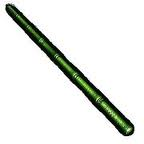
\includegraphics[width=.2\textwidth]{stick}}
    \caption[打狗棒]{\label{fig:stick} 打狗棒}
\end{figure}

\subsection{惡狗攔路}

举棒横在身前,待敌兵器击到,侧抖旁缠,顺势借力向外斜甩,将敌兵器掠在一旁。
\begin{listing}[H]
  \begin{minted}[fontsize=\small,
    linenos=true,numbersep=10pt,
    frame=lines,framesep=10pt,rulecolor=\color{lightgray},
    xleftmargin=4cm, xrightmargin=4cm,
    gobble=4,
    ]{python}
    while true:
        run
  \end{minted}
  \caption{恶狗拦路Python应用示例}
  \label{lst:run}
\end{listing}
恶狗拦路的应用示例如程序~\ref{lst:run}所示。

\subsection{棒打雙犬}
以迅猛之势横扫敌双足。具体应用如程序~\ref{lst:cry}所示。

\begin{listing}[H]
  \begin{minted}[fontsize=\small,
    linenos=true,numbersep=10pt,
    frame=lines,framesep=10pt,rulecolor=\color{lightgray},
    xleftmargin=4cm,xrightmargin=4cm,
    gobble=4,
    ]{c}
    while(dogs == 2){
      cry();
    }
  \end{minted}
  \caption{棒打双犬C应用示例}
  \label{lst:cry}
\end{listing}

\subsection{斜打狗背}
棒身倏地伸出,棒头搭在敌兵器上,轻轻向下按落,以四两拨千斤之理出招。

\subsection{撥狗朝天}
棒身伸出,将敌兵器前端挑甩上来。

\subsection{獒口奪杖}
在竹棒被敌夺去後,伸右手食中二指取敌双目,同时左足翻起,压住棒身,立时夺回,此招变幻莫测,
夺棒时百发百中,纵是武功高已数倍之敌,亦难保全。 

\subsection{棒打狗頭}
以迅猛之势向敌头顶击去。

\subsection{反戳狗臀}
棒身横扫敌臀部。

\subsection{棒挑癩犬}
敌抓住棒身时,前伸斜掠,将棒身挑出。

\subsection{壓扁狗背}
棒身倏地伸出,棒头搭在敌兵器上,轻轻向下按落,以四两拨千斤之理出招。

\subsection{天下無狗}
共有六变,是打狗棒法最后一招最后一变最精妙的绝招,这一招仗将出来,四面八方是棒,劲力所至,
令人难以抵挡,便有几十条恶犬也一齐打死了,所谓“天下无狗”便是此义,棒法之精妙,已臻武学中的
绝诣。

\section{口诀}

\begin{description}
\item[挑字诀:] 棒挑癞犬 歹挑狗身 捣乱狗窝 挑拨狗爪
\item[封字决:] 压扁狗背 饿狗拦路 犬牙交错 母狗护雏   
\item[转字决:] 恶犬回咬 快击狗臀 丧家之犬 黄狗追尾 幼犬戏球   
\item[绊字诀:] 獒口夺杖 拨狗朝天 横打双獒 鸡飞狗跳   
\item[引字诀:] 引狗入寨 棒迥掠地 斜打狗背 摇头摆尾 群狗争食   
\item[戳字诀:] 歹戳狗臀 狗急跳墙 蜀犬吠日 狗眼看人   
\item[缠字诀:] 斗犬十弄 棒打双犬 死拉狗尾 狗咬狗骨 老狗乞怜   
\item[劈字诀:] 棒打狗头 穷巷赶狗 疯狗咬喉 落水打狗 天下无狗
\end{description}

%%% Local Variables: 
%%% mode: latex
%%% TeX-master: "../sample"
%%% End: 
